\documentclass[12pt,letterpaper,titlepage]{article}

\usepackage{fontspec}
\defaultfontfeatures{Mapping=tex-text}
\usepackage{xunicode}
\usepackage{xltxtra}
\usepackage{amsmath}
\usepackage{pdfpages}
\usepackage{amsfonts}
\usepackage{bbold}
\usepackage{amssymb}
\setcounter{secnumdepth}{0}
\usepackage{nameref}
\usepackage{enumitem}
\usepackage{environ}
\usepackage{pgfplots}
\usepackage{listings}

\showboxdepth=\maxdimen
\showboxbreadth=\maxdimen


\usepackage{paracol}
\usepackage{wrapfig}
\globalcounter{table}
\globalcounter{figure}
\usepackage{graphicx}
\usepackage[left=1in,right=1in,top=1in,bottom=1in]{geometry}
\graphicspath{{img/}}

\author{Jacob Abel}
\title{	Design \& Simulate 13
	\\\large ECE2204 CRN:82929
}

\setlength{\parskip}{0.5em}

\begin{document}
\maketitle
\begin{raggedright}

\section{Problem 13.3-4.a.1: } Added $R_S$ and shuffled values.
\subsection{Design}

For the circuit below assume $R_1 = 80k\Omega$, $R_2 = 120k\Omega$, $R_D = 200k\Omega$, $V_{DD} = 12V$, $V_{TP} = -1V$, and $K_P = 0.15 mA/V^2$. Add a source resistor $R_S$ and design the system to place the transistor in border mode.

\begin{center}
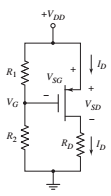
\includegraphics[width=\textwidth, height=12\baselineskip, keepaspectratio=true]{ds1}
\end{center}

As the transistor is in border mode, $V_{DG} = |V_T| \implies V_{GD} = -|V_T|$.

\begin{align*}
   V_G
     &= \frac{R_2}{R_1 + R_2}(V_{DD})
      = \frac{120k\Omega}{200k\Omega}(12V)
      = 7.2V
\\ V_{GD}
	 &= -|V_T|
	  = -1V
\\ V_D
	 &= V_G + V_{GD}
	  = 7.2V + 1V
	  = 8.2V
\\ I_D
	 &= \frac{V_D}{R_D}
	  = \frac{8.2V}{200k\Omega}
	  = 41\mu A
\\ V_{SG}
	 &= \sqrt{\frac{I_D}{K_p}} - V_{TP}
	  = \sqrt{\frac{41\mu A}{0.15 mA/V^2}} + 1V
	  = 1.523V
\\ V_{S}
	 &= V_G + V_{SG}
	  = 7.2V + 1.523V
	  = 8.72V
\\ R_S
	 &= \frac{V_{DD} - V_{S}}{I_D}
	  = \frac{12V - 8.72V}{41 \mu A}
	  = 80k\Omega
\end{align*}

The source resistor value is $R_S = 80k\Omega$.

\clearpage
\subsection{Validation}

\begin{center}
LTSpice Implementation (Simulated Values within $<1\%$)
\columnratio{0.5}
\begin{paracol}{2}
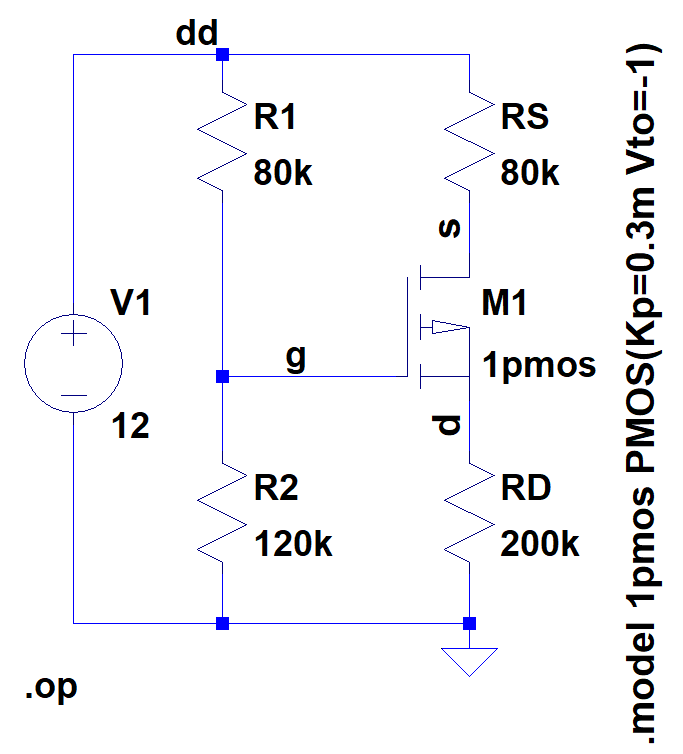
\includegraphics[width=.48\textwidth, height=\textheight, keepaspectratio=true]{ds1b}
\switchcolumn
\begin{tabular}{|l|l|c|}
  \hline V(dd):	    & 12	        & voltage
\\\hline V(g):	    & 7.2	        & voltage
\\\hline V(s):	    & 8.7122	    & voltage
\\\hline V(d):	    & 8.21949	    & voltage
\\\hline Id(M1):	& 4.11705e-005	& device\_current
\\\hline Ig(M1):	& -0	        & device\_current
\\\hline Ib(M1):	& -1.87487e-006	& device\_current
\\\hline Is(M1):	& -3.92956e-005	& device\_current
\\\hline I(Rd):	    & 4.10975e-005	& device\_current
\\\hline I(Rs):	    & 4.10975e-005	& device\_current
\\\hline I(R2):	    & 6e-005	    & device\_current
\\\hline I(R1):	    & 6e-005	    & device\_current
\\\hline I(V1):	    & -0.000101097	& device\_current
\\\hline
\end{tabular}
\end{paracol}
\begin{align*}
   Err_{V_S} &= \frac{|8.72-8.7122|}{8.72} = 0.00089 = 0.09\%
\\ Err_{V_D} &= \frac{|8.2-8.219|}{8.2} = 0.00231 = 0.23\%
\\ Err_{I_D} &= \frac{|41-41.17|}{41} = 0.00414 = 0.41\%
\end{align*}
\end{center}

\clearpage
\section{Problem 13.3-4.b.1: } Adapted from Problem 3.26 on page 197 by changing some values, switching eNMOS to ePMOS.
\subsection{Design}

Considering the circuit below, assume that the transistor is instead an ePMOS, $R_S$ and $R_D$ are swapped, $V_{TP} = -0.75V$, $K_p = 0.25 mA/V^2$, and $V_{DD} = 12V$. Calculate $V_{SG}$, $I_D$, and $V_{SD}$.

\begin{center}
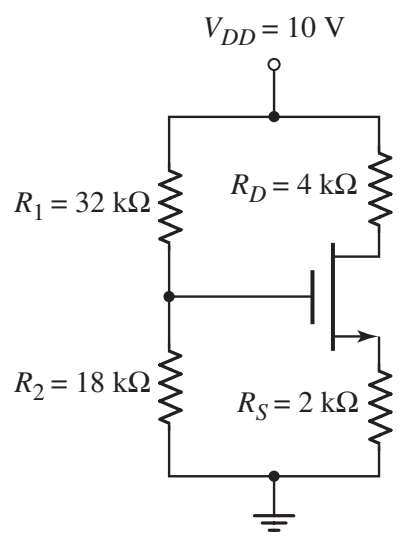
\includegraphics[width=\textwidth, height=12\baselineskip, keepaspectratio=true]{ds2}
\end{center}

\begin{align*}
   V_G
    &= \frac{R_2}{R_1 + R_2}(V_DD)
     = \frac{18k\Omega}{32k\Omega+18k\Omega}(12V)
     = 4.32V
\\ V_{SG}
    &= V_{DD} - I_DR_S - V_G
     = 12V - 4.32V - 2k\Omega I_D
     = 7.68V - 2k\Omega I_D
\\ I_D
	&= K_p (V_{SG} + V_{TP})^2
	 = (0.25 mA/V^2) (7.68V - 2k\Omega I_D - 0.75V)^2
\\	&= 2.0375mA\text{ OR } 5.8923mA
\\ V_{DD}
	&= V_D + V_{SD} + V_{S}
	 = V_{SD} + I_DR_S + I_DR_D
	 = V_{SD} + I_D(R_S + R_D)
\\ V_{SD}(sat)
	&= V_{SG} + V_{TP}
\\	&= 7.68V - 2k\Omega (2.0375mA) - 0.75V
	 = 2.85V
\\  &= 7.68V - 2k\Omega (5.8923mA) - 0.75V
     = -4.85V
\\ V_{SD}
	&= V_{DD} - I_D(R_S + R_D)
\\  &= 12V - (2.0375mA)(2k\Omega + 4k\Omega)
	 = -0.225V
\\  &= 12V - (5.8923mA)(2k\Omega + 4k\Omega)
	 = -23.354V
\end{align*}

$V_{SD} < V_{SD}(\text{sat})$ and therefore the transistor is in the non-saturation region.

\begin{align*}
   I_D
  	&= K_p [2V_{SD}(V_{SG} + V_{TP}) - V_{SD}^2]
\\	&= (0.25 mA/V^2)[2(12V - 6k\Omega I_D)(7.68V - 2k\Omega I_D - 0.75V) - (12V - 6k\Omega I_D)^2]
\\	&= 1.78101mA \text{ OR } -1.04435mA
\\ V_{SD}
\\  &= 12V - (1.78101mA)(2k\Omega + 4k\Omega)
	 = 1.314V
\\  &= 12V + (1.04435mA)(2k\Omega + 4k\Omega)
	 = 18.266V
\end{align*}

\begin{align*}
   I_D 
	&= 1.78101mA
\\ V_{SG}
	&= 7.68V - 2k\Omega(1.78101mA)
	 = 4.118V
\\ V_{SD}
    &= 12V - (1.78101mA)(2k\Omega + 4k\Omega)
	 = 1.314V
\\ V_S
	&= V_G + V_{SG}
	 = 4.32V + 4.118V
	 = 8.438V
\\ V_D
	&= V_S - V_{SD}
	 = 8.438V - 1.314V
	 = 7.124V
\end{align*}

\clearpage
\subsection{Validation}

\begin{center}
LTSpice Implementation
\columnratio{0.52}
\begin{paracol}{2}
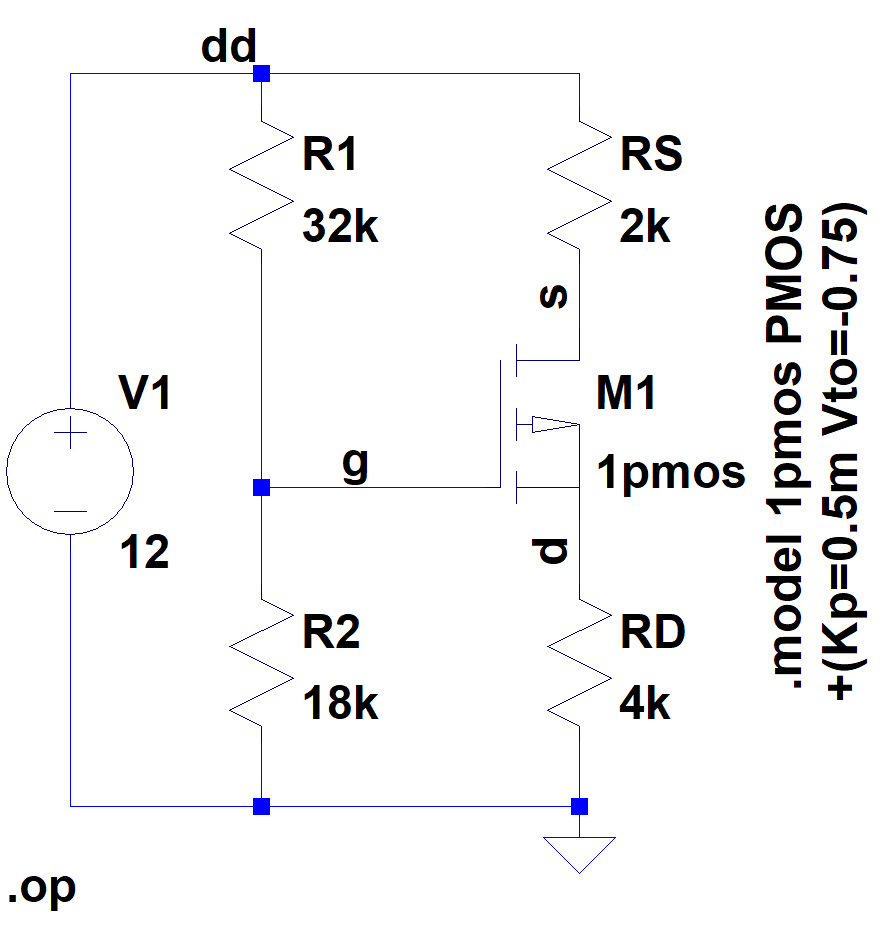
\includegraphics[width=.5\textwidth, height=\textheight, keepaspectratio=true]{ds2b}
\switchcolumn
\begin{tabular}{|l|l|c|}
  \hline V(dd):	 & 12	        & voltage
\\\hline V(g):	 & 4.32	        & voltage
\\\hline V(s):	 & 8.2186	    & voltage
\\\hline V(d):	 & 7.56279	    & voltage
\\\hline Id(M1): & 0.00195211	& device\_current
\\\hline Ig(M1): & -0	        & device\_current
\\\hline Ib(M1): & -0.00102718	& device\_current
\\\hline Is(M1): & -0.000924925	& device\_current
\\\hline I(Rd):	 & 0.0018907	& device\_current
\\\hline I(Rs):	 & 0.0018907	& device\_current
\\\hline I(R2):	 & 0.00024	    & device\_current
\\\hline I(R1):	 & 0.00024	    & device\_current
\\\hline I(V1):	 & -0.0021307	& device\_current
\\\hline
\end{tabular}
\end{paracol}
\begin{align*}
   Err_{V_S} &= \frac{|8.438-8.2186|}{8.438} = 0.0262 = 2.62\%
\\ Err_{V_D} &= \frac{|7.124-7.5629|}{7.124} = 0.0616 = 6.16\%
\\ Err_{V_G} &= \frac{|4.32-4.32|}{4.32} = 0 = 0.00\%
\\ Err_{I_D} &= \frac{|1.78101-1.8907|}{1.78101} = 0.0615 = 6.15\%
\end{align*}

The deviation in values is likely due to a minor mistake in the work performed during calculation of results. I spent a long time looking for it but I was unable to find it. 
\end{center}

This assignment should demonstrate a basic understanding of DC Biased MOSFET circuits.

\textit{I have neither given nor received unauthorized assistance on this assignment.}


\end{raggedright}
\end{document}
